\chapter[\textsl{Rasa} Theory: Changes and Growth]{\textsl{Rasa} Theory: Changes and Growth}\label{chapter\thechapter:begin}
%~ \footnotetext[1]{pp.~\pageref{chapter\thechapter:begin}--\pageref{chapter\thechapter:end}. In: Kannan, K S (Ed.) (2018) {\sl Śāstra-s Through the Lens of Western Indology - A Response}. Chennai: Infinity Foundation India.}
\Authorline{Naresh P. Cuntoor}
\lhead[\small\thepage\quad Naresh P. Cuntoor]{}
\index{rasa theory@\textsl{rasa} theory}

\section*{Introduction}

\textsl{Rasa}\index{rasa@\textsl{rasa}} has been a significant area of interest over several centuries in Indian literary analysis. From Bharata\index{Bharata} to modern day Sanskrit scholars, the theory of \textsl{rasa} has been studied under the formalisms of Mīmāṁsā,\index{Mimamsa@Mīmāṁsā} Vedānta\index{Vedanta Tradition@Vedānta Tradition} and Bhakti\index{Bhakti Tradition} traditions. The formalisms have sharpened our understanding of the contribution of \textsl{rasa} theorists. As a result of the insight gained through analysis, we are often better-equipped to appreciate the poet’s imagination. The primacy of \textsl{rasa} has been debated in the context of several concepts of literary analysis such as \textsl{alaṅkāra}, \textsl{dhvani} and \textsl{aucitya}. It is thus unsurprising that \textsl{rasa }has attracted Pollock’s attention, whose works in several Sanskrit-related topics have been influential. This paper has two main objectives: to summarize Pollock’s perspectives on \textsl{rasa}\index{rasa theory@\textsl{rasa} theory} theory, and to outline areas of study in modern cognitive and computational aesthetics.\index{computational aesthetics} The latter is motivated by the discussion of the science and history of \textsl{rasa}\index{rasa@\textsl{rasa}} in Pollock (2012). Insofar as the first objective is concerned, only the main arguments related to Pollockian claims are discussed. Lengthy quotations are avoided for the sake of brevity (without hopefully, sacrificing clarity). 

At the outset, we have identified three broad themes for discussion: the evolution of \textsl{rasa}, the formalisms used to describe \textsl{rasa}, and the discussion of science and history of \textsl{rasa}. There are other themes that merit investigation as well. In particular, it may be interesting to discuss the aims of \textsl{rasa} and how the evolution of the types of \hbox{\textsl{rasa}-s} and \textsl{bhāva}-s\index{bhava@\textsl{bhāva}} may contribute to changes in aims of \textsl{rasa}. Further, the ways of depicting \textsl{rasa} and potential flaws in its depiction may merit closer study. Both these aspects are addressed in Pollock’s writings. We chose to focus on the three themes of \textsl{rasa}\index{rasa@\textsl{rasa}} evolution, formalism and \textsl{rasa}-related science to limit the scope of the paper. The paper is organized into three sections. Section 1 discusses three types of changes and their impact on societal and cultural constructs. Section 2 describes the different frameworks under which \textsl{rasa}\index{rasa@\textsl{rasa}} has been described, and their implications. Drawing from cognitive neuroscience, computational aesthetics,\index{computational aesthetics} reductionism\index{reductionism} and Pollock’s analysis, Section 3 discusses potential future work in the context of \textsl{rasa}\index{rasa theory@\textsl{rasa} theory} theory. The paper concludes with questions that may merit response from traditional Sanskrit scholars to address Pollock’s analysis.\\[-20pt]

\section*{\textsl{Rasa} through the Prism of Change}
\index{rasa@\textsl{rasa}}

A recurring theme in Pollock’s treatment of \textsl{rasa} seeks to identify revolutionary changes in the development of the theory. Revolutionary changes, real or hypothesized, are highlighted more strongly than gradual, evolutionary and natural changes. Some of these discussions are echoed in discussions of Sanskrit in Pollock (2006) as well. A few examples of the changes discussed are discussed below:
\begin{enumerate}
\itemsep=0pt
\item Fundamental differences between literature-seen and literature-heard, and their implications on \textsl{rasa }
\item Expression of \textsl{rasa} in sense of \textsl{rasa}-laden statements to its full realization
\item Change in \textsl{rasa} localization
\end{enumerate}

\section*{Changes from Drama to Poetry}

One of the main elements of Pollock’s \textsl{rasa}\index{rasa@\textsl{rasa}} analysis is the identification of a “fundamental” difference between literature-seen and literature-heard (\textsl{dṛśya-kāvya}\index{drsyakavya@\textsl{dṛśyakāvya}} and \textsl{śrvya-kāvya}).\index{sravyakavya@\textsl{śravyakāvya}} The distinction and its implication on \textsl{rasa} theory\index{rasa theory@\textsl{rasa} theory} is developed in several steps as outlined below (Pollock, 2012):
\begin{enumerate}
\itemsep=1pt
\item Sanskrit texts themselves recognize the two forms of literature (seen and heard). 
\item The two forms are said to be fundamentally different so that they require different forms of analysis.
\item \textsl{Rasa }analysis in Sanskrit literature began with literature-seen.
\item \textsl{Rasa }analysis eventually evolved so that it could be applied to literature-heard.
\item The analytical evolution of \textsl{rasa} from literature-seen to literature-heard should have required significant development in \textsl{rasa} theory.\index{rasa theory@\textsl{rasa} theory} The steps and characteristics of evolution have thus to be identified.
\end{enumerate}

The key points used to substantiate the above set of arguments are described next, beginning with Pollock (2012)’s claim that the two forms of literature are fundamentally different. This is a key assumption upon which Pollock’s change-based perspective of the evolution of \textsl{rasa} theory\index{rasa theory@\textsl{rasa} theory} is built. The differences need to be fundamental and significant enough to merit a separate analysis of \textsl{rasa} theory for the two forms of literature. If the difference is merely superficial, then it would be difficult to assert the main claim of Pollock (2012) which is that the development of \textsl{rasa} theory required a substantial change --- substantial enough to merit a change in \textsl{rasa }ontology and epistemology --- to the theory. 

\section*{Evidence for Fundamental Difference between Literary Forms}

Three specific instances are offered as proof of fundamental difference between the two forms of literature. Firstly, Bhoja\index{Bhoja} recognizes that \textsl{rasa}\index{rasa@\textsl{rasa}} is present in both literature-seen and literature-heard (\textsl{Śṛṅgāraprakāśa},\index{Srngaraprakasa@\textsl{Śṛṅgāraprakāśa}} 1.12). Moreover, Pollock (2012) opines that “...not only were the two genres categorically differentiated; they were often radically opposed…” To justify the claim, Bhoja’s remarks in \textsl{Śṛṅgāraprakāśa} (1.12) are presented. Here, Bhoja\index{Bhoja} considers poets and \textsl{kāvya }to be more praiseworthy than actors and acting. Whereas actors can portray \textsl{rasa} right before one’s eyes, poets allow the audience to experience the \textsl{kāvya }more fully. 

Secondly, Pollock (2012) quotes an anonymous verse which has been “cited by Śrīdhara while restating Bhoja’s view” to provide a stronger reason for treating \textsl{rasa} in literature-heard as superior to that of literature-seen, viz., the range of narrative power in literature-heard. 
Thirdly, Abhinavagupta’s\index{Abhinavagupta} diametrically opposite view in \textsl{Abhinavabhāratī},\index{Abhinavabharati@\textsl{Abhinavabhāratī}} which takes the side of actors over poets, is discussed. Being a commentary on the \textsl{Nāṭyaśāstra}, it is natural to expect a biased treatment of actors and acting. But Pollock (2012) does not explain why this bias should be discounted. Instead, it quotes Abhinavagupta explaining his justification for holding drama (in any of its ten forms) as the best literary form. 

It is indeed interesting to understand how the difference in perspectives held by Bhoja\index{Bhoja} and Abhinavagupta,\index{Abhinavagupta} even when seen in the context of their own literary biases, can provide insight into different forms of literature. That is not the context within which we encounter the discussion of the two literary forms in Pollock (2012). At any rate, based on the three reasons described above, Pollock (2012) asserts the fundamental difference in the two forms of literature before turning to the development of \textsl{rasa}.\index{rasa@\textsl{rasa}} 

If there is a fundamental difference in the literary forms, then their \textsl{rasa}\index{rasa@\textsl{rasa}} analysis must also be different. With its greater range of narrative capability, Pollock (2012) argues that literature-heard can support \textsl{rasa}\index{rasa@\textsl{rasa}} development that literature-heard cannot. In particular, an increase in the number of \textsl{rasa}s is offered as a direct consequence of the extension of literature-seen \textsl{rasa }to literature-heard \textsl{rasa}. The dispute over the number of \textsl{rasa}-s is then described in the context of the hypothesized extension in \textsl{rasa} theory.\index{rasa theory@\textsl{rasa} theory}

Before turning to the implications of differences in the two literary forms on \textsl{rasa} theory, it is instructive to read Bhoja’s\index{Bhoja} comments in context which is not provided in Pollock (2012). Bhoja considers \textsl{sāhitya} to be more praiseworthy than word and meaning, and then goes on to describe the relationship between the two. Seen in this context, Bhoja’s comments may be seen as a discussion of difference between the visible and beyond-visible entities. Seen in context, it is difficult to arrive at Pollock (2012)’s conclusion that Bhoja\index{Bhoja}
 recognized a fundamental difference between the two forms of literature.

\section*{Differences in Literary Forms and their Implication on \textsl{Rasa} Theory}
\index{rasa theory@\textsl{rasa} theory}

The oldest extant text on dramaturgy in India, Bharata’s\index{Bharata} \textsl{Nāṭyaśāstra} discusses virtually every component of dramatic performance including actors and audience, acting and theatrical devices, and language and suitability. Pollock (2016) describes Bharata’s contribution and reminds the reader about long-standing questions that have occupied traditional scholars. The questions include the seemingly “disconne\-cted components” of \textsl{bhāva}-s\index{bhava@\textsl{bhāva}} and related factors, the number of \textsl{rasa}-s,\index{rasa@\textsl{rasa}} and the localization of \textsl{rasa}.

In context of his treatise, Bharata\index{Bharata} describes the types and characteristics of \textsl{rasa}-s. But he does not consider the question of whether \textsl{rasa} was the exclusive domain of drama. Having asserted that the distinction between literature-seen and literature-heard was “clearly established from a relatively early date,” Pollock (2012) goes on identify Rudrabhaṭṭa\index{Rudrabhatta@Rudrabhaṭṭa} (circa 10th c. CE) as the first and only in the tradition to infer the development of \textsl{rasa}\index{rasa@\textsl{rasa}} from drama to poetry. 

Between Bharata\index{Bharata} and Rudrabhaṭṭa, Pollock (2012) and Pollock (2016) discusses the role of poets and theorists such as Daṇḍin,\index{Dandin@Daṇḍin} Bhāmaha\index{Bhamaha@Bhāmaha} and Rudraṭa\index{Rudrata@Rudraṭa} in the development of \textsl{rasa}.\index{rasa@\textsl{rasa}} It concludes that in the view of Bhāmaha and Daṇḍin, the representation of emotion is secondary to \textsl{alaṅkāra}-s. In this intervening period between Bharata\index{Bharata} and Rudrabhaṭṭa,\index{Rudrabhatta@Rudrabhaṭṭa} Udbhaṭa\index{Udbhata@Udbhaṭa} is hailed as the most significant \textsl{rasa} theorist. 

\section*{Changes in \textsl{Rasa} Expression}
\index{rasa@\textsl{rasa}}

In Pollock (2016), Udbhaṭa’s treatment of \textsl{rasa} is said to be a final blow to the existing notions of \textsl{rasa} expression. This is indeed a valuable insight to gain if it stands to scrutiny. Next we shall describe the arguments presented in Pollock (2016) to highlight Udbhaṭa’s\index{Udbhata@Udbhaṭa} role: 

\begin{myquote}
Udbhaṭa’s treatment of aesthetic emotion marks the final—and by now contradiction-riddled—stage where the conceptual framework of the older rhetorical analysis … was stressed to the breaking point. And Udbhaṭa nearly broke it. He radically redefines the earlier notions of Bhāmaha\index{Bhamaha@Bhāmaha} and Daṇḍin,\index{Dandin@Daṇḍin} formulated when dramaturgical \textsl{rasa}\index{rasa theory@\textsl{rasa} theory} theory had yet to be fully adapted to poetry, and masterfully assimilates them to … the classical typology... Thus, the ornament known as the “\textsl{rasa}-laden” statement, earlier viewed as heightened or climactic emotion, now explicitly becomes the “full realization” of \textsl{rasa}, with the complete panoply of aesthetic elements (the foundational and stimulant factors, and the rest).\hfill Pollock (2016:73)
\end{myquote}

Now let us see how the prior “contradiction-riddled” stage is described. The treatment of \textsl{rasa} by Bharata,\index{Bharata} Bhāmaha and Daṇḍin are presented as follows. Pollock (2016) quotes Bharat’s view as “\textsl{rasa} arises from the conjunction of factors, reactions, and transitory emotions,” and gives the taste analogy used to explain \textsl{rasa}.\index{rasa@\textsl{rasa}} Then, Bharata discusses why only stable emotions become \textsl{rasa}s, and concludes that "Stable emotions become the master, and the transitory emotions become subservient..." 

\begin{myquote}
[343] Here one might ask: If the \textsl{rasa}s arise from the forty-nine emotions connected with the subject matter of a literary work, when these emotions are manifested by the factors and the physical reactions in combination with their common properties, why is it only the stable emotions that are said to become \textsl{rasa}s? Our answer is as follows: Just as human beings, despite the fact that they have common physical traits, similar hands and feet and torsos and frames, and common major and minor limbs, will become, some of them, kings by reason of their family...

\hfill Pollock (2016:64)
\end{myquote}

Then, Bharata\index{Bharata} discusses the role of psychic sensitivity:

\begin{myquote}
[373.3] Here one might ask whether the acting out of the other emotions is supposed to happen without psychic sensitivity, such that only these responses should be called psychophysical. My answer is as follows. Psychic sensitivity as defined here is something that arises from the mind; it is said to be the mind in a state of heightened awareness, since the psychic sensitivity arises when the mind is thus aware.

\hfill Pollock (2016:65)
\end{myquote}

After quoting the above discussions of Bharata,\index{Bharata} Pollock (2016) mentions that Bhāmaha\index{Bhamaha@Bhāmaha} took “a radically different view.” The difference seems to be that Bhāmaha “does not even treat \textsl{rasa} as a separate topic” in his work on poetics, or more precisely, ornamentation. The lack of treatment of \textsl{rasa}\index{rasa@\textsl{rasa}} is said to be symptomatic of a lack of clear conceptualization of \textsl{rasa}. Had the significance of \textsl{rasa} expression been understood more clearly, the argument goes, the emotion tropes of Bhāmaha would have captured \textsl{rasa} more fully instead of discussing a list of ornaments. A similar criticism is made of Daṇḍin\index{Dandin@Daṇḍin} as well. However, Daṇḍin clearly recognizes \textsl{rasa}-s as described by Bharata.\index{Bharata} 

This is said to be the contradiction-riddled stage which led to a clear break with Udbhaṭa.\index{Udbhata@Udbhaṭa} It would be interesting to get a clearer understanding of contradictions in \textsl{rasa}\index{rasa theory@\textsl{rasa} theory} theory at the time of Udbhaṭa, and how they were resolved in Udbhaṭa’s treatment. 

\section*{Change in the localization of \textsl{rasa}}

In describing Bhaṭṭa Nāyaka’s\index{Bhattanayaka@Bhaṭṭa Nāyaka} contribution to \textsl{rasa }theory, Pollock (2009) begins by recounting the prevalent consensus of \textsl{rasa}\index{rasa@\textsl{rasa}} as “a phenomenon pertaining to the characters, not the spectators. In this conception, \textsl{rasa }meant the emotional response in the hero or heroine.” Pollock (2009) does not try to show a monotonic change from \textsl{rasa} as something that pertains to characters to something that pertains to the audience. Instead it traces a checkered history of various theorists’ description of \textsl{rasa} localization. I shall briefly recount that description next. 

According to Bhaṭṭa Lollaṭa,\index{Bhattalollata@Bhaṭṭa Lollaṭa} \textsl{rasa} is something that “comes into being” in the characters. “Śrī Śaṅkuka\index{Sankuka@Śaṅkuka} was the first to argue from the spectators’ point of view” to a certain extent when he propounded the \textsl{anumatipakṣa}, which takes the position that \textsl{rasa} can only be inferred from the imitation of drama. Dhanañjaya\index{Dhananjaya@Dhanañjaya} and Dhanika\index{Dhanika} however, state much more clearly that \textsl{rasa} belongs to the spectator experiencing the \textsl{rasa}, because he is alive and present, and not to the character. Bhaṭṭa Nāyaka\index{Bhattanayaka@Bhaṭṭa Nāyaka} then uses the framework of Mīmāṁsā\index{Mimamsa@Mīmāṁsā} to describe his \textsl{rasa} theory\index{rasa theory@\textsl{rasa} theory} (Pollock, 2009). 
Pollock (2009) makes a strong case for Bhaṭṭa Nāyaka’s contribution in localizing \textsl{rasa}\index{rasa@\textsl{rasa}} in the spectator, using his notion of \textsl{bhāvanā}\index{bhavana@\textsl{bhāvanā}} as a literary phenomenon. This discussion relies mostly on the characterization of theorists who followed him because Bhaṭṭa Nāyaka’s\index{Bhattanayaka@Bhaṭṭa Nāyaka} original writings are sparsely available. 

While highlighting Bhaṭṭa Nāyaka’s contribution however, several factors are not discussed, though they are mentioned elsewhere. I shall mention three factors. Firstly, the role of the audience is clearly recognized in the \textsl{Nāṭyaśāstra} itself which discusses the different types of audience in chapter 27. Had the focus of drama and \textsl{rasa}\index{rasa@\textsl{rasa}} been on the characters themselves, it may be argued that the discussion of audience and their varying levels of comfort are superfluous. Secondly, Śaṅkuka’s\index{Sankuka@Śaṅkuka} example of painted horse which is mentioned in Pollock (2016:82) is described perhaps as the first instance of applying the notion of \textsl{rasa} across poetry and painting. It would seem that such an application across art disciplines is more striking than application across two forms of literature, drama and poetry. So the reader would be interested to understand the primacy of \textsl{rasa}\index{rasa@\textsl{rasa}} extension of drama to poetry, over that of painting. Thirdly, let us consider the following position of Śaṅkuka: 

\vskip .1cm

\begin{myquote}
When the sage states, “Whether rasa precedes emotion or emotion rasa is a function of the nature of the case: in the course of a dramatic performance, while relishing the rasa in the actor, viewers apprehend the stable emotion in the character,” he is affirming the first option. In the actual world depicted in the drama, however, it is as a result of the character’s first seeing “emotion” that its essential form, namely rasa, arises.]
\hfill Pollock (2016:85)
\end{myquote}

\vskip .1cm

Here Mammaṭa\index{Mammata@Mammaṭa} recounts Śaṅkuka’s\index{Sankuka@Śaṅkuka} position as follows:

\vskip .1cm

\begin{myquote}
Shri Śaṅkuka’s position is as follows. The stable emotion is inferred to exist in the actor, whom we grasp by a mode of comprehension different from all four normal forms of apprehension…. This inference arises from a “conjunction”—that is, an inferential relationship—of three elements: (1) a cause, which is designated by the term “foundational and stimulant factor”; (2) an effect, which is designated by the term “reaction”; (3) an auxiliary cause, which is designated by the term “transitory emotion.” The first is distinctly comprehended from the literary narration itself, such as in the following verse, where we have a foundational factor for the erotic rasa enjoyed.
\hfill Pollock (2016:85)
\end{myquote}

\vskip .1cm

In this section, it is clear that the viewers are responding to the dramatic performance as depicted by the actor. And Śaṅkuka\index{Sankuka@Śaṅkuka} gives a possible explanation of the relationship between \textsl{rasa} and the stable emotion. He closes by noting that “the erotic \textsl{rasa}\index{rasa@\textsl{rasa}} is enjoyed.” In other examples, other \textsl{rasa-}s are similarly discussed. From the context of the commentary, it seems that the \textsl{rasa} is enjoyed by the viewers. If that is not the case, a detailed discussion of Śaṅkuka’s and others’ arguments would merit a thorough examination before asserting a clean break between \textsl{rasa} in characters and \textsl{rasa} in viewers. 

\section*{Consequence of Shifting \textsl{Rasa} Localization}

One of the consequences of localizing \textsl{rasa}\index{rasa@\textsl{rasa}} in the viewer rather than the character is that questions of manifestation or creation are rendered moot. However that still leaves the question of how \textsl{rasa} is recognized by the reader. In the context of Ānandavardhana,\index{Anandavardhana@Ānandavardhana} Pollock (2016) describes how its consideration is missing thus: 

\begin{myquote}
More important, he never addresses the question of how the reader knows or experiences it. We are justified in inferring from this loud silence that for Ananda, none of these questions mattered, and that the phenomenon of \textsl{rasa} was basically unproblematic. He conceived of it as his predecessors had; the great insights that would transform aesthetic theory were a generation away. For all his remarkable insight into how literary meaning is engendered, Ananda plainly had no interest in how it was experienced, and in this he conformed to the formalistic analysis that he inherited.
\hfill Pollock (2016:89)
\end{myquote}

This is a question that was considered by Mahima Bhaṭṭa\index{Mahimabhatta@Mahimabhaṭṭa} as noted below.

\begin{myquote}
Mahima agrees that in the final analysis \textsl{rasa}\index{rasa@\textsl{rasa}} is an “experience of rapture on the part of the responsive viewer/reader,” but the only possible application of the term “manifestation” to that process, he argues, is a figurative one. What actually happens is that we infer \textsl{rasa} from the aesthetic elements; hence, though these elements do not “manifest” \textsl{rasa}, the use of “manifestation” in a figurative sense may be allowed as pointing toward the uniqueness of the final experience. It is toward establishing the limits of this figurative usage of “manifestation,” in addition to denying its literal use in favor of inference, that Mahima Bhaṭṭa’s efforts here are directed.
\hfill Pollock (2016:103)
\end{myquote}

Further, Pollock (2016) corrects Jagannātha’s\index{Jagannatha@Jagannātha} understanding of Bhaṭṭa Nāyaka’s\index{Bhattanayaka@Bhaṭṭa Nāyaka} contribution as follows:

\begin{myquote}
Jagannātha argued that Bhaṭṭa Nāyaka’s “experientialization” is no different from the doctrine of “manifestation,” he was correct but had things reversed: “manifestation” became no different from “experientialization” once the original doctrine of Ānandavardhana,\index{Anandavardhana@Ānandavardhana} designed to explain the linguistic phenomenon of \textsl{rasa},\index{rasa@\textsl{rasa}} had been recoded by Abhinavagupta\index{Abhinavagupta} into something intended to approximate experientialization, thanks to his appropriation of Bhaṭṭa Nāyaka’s own doctrines.
\hfill Pollock (2016:134)
\end{myquote}

\newpage

It is interesting to note that considerations of stable emotions and \textsl{rasa} find clear resonance in current research in sentiment analysis and opinion mining (Liu, 2012). Building on the analysis of Pollock (2016), it is possible that further study based on computational techniques could shed further light on the contribution of the shift in \textsl{rasa} localization.\\[-20pt] 

\section*{\textsl{Rasa} Seen Through Different Formalisms}

Over time, \textsl{rasa}\index{rasa theory@\textsl{rasa} theory} theory came to be expounded under the framework of different formalisms. Pollock delves in details of a few frameworks including Mīmāṁsā,\index{Mimamsa@Mīmāṁsā} Vedānta\index{Vedanta Tradition@Vedānta Tradition} and the Bhakti\index{Bhakti Tradition} movement.\\[-20pt]

\section*{Mīmāṁsā Framework}

The Mīmāṁsā framework of \textsl{rasa} theory is largely credited to Bhaṭṭa Nāyaka’s\index{Bhattanayaka@Bhaṭṭa Nāyaka} and Abhinavagupta’s\index{Abhinavagupta} \textsl{rasa} theories (Pollock (2009), Pollock (2016)). The three elements of Mīmāṁsā\index{Mimamsa@Mīmāṁsā} Shastra, viz., \textsl{sādhya},\index{sadhya@\textsl{sādhya}} \textsl{sādhana}\index{sadhana@\textsl{sādhana}} and \textsl{itikartavyatā},\index{itikartavyata@\textsl{itikartavyatā}} for analyzing a scriptural statement are described as follows: (1) what is to be produced by action, (2) whereby it is to be produced, and (3) how it is to be produced. Based on the available fragments of Bhaṭṭa Nāyaka’s work (and subsequent commentators’ descriptions of Bhaṭṭa Nāyaka), Pollock (2009) surmises that he extended the Mīmāṁsā analytical framework to literature. 

Pollock (2009) takes up the difficult task of analyzing Mīmāṁsā’s\index{Mimamsa@Mīmāṁsā} influence on Bhaṭṭa Nāyaka.\index{Bhattanayaka@Bhaṭṭa Nāyaka} The difficulty arises because of two main reasons - Bhaṭṭa Nāyaka’s writings are available in scattered fragments that do not lend themselves to forming a complete picture of his theory, and his personal philosophical allegiance is unknown. We do not know the type of Mīmāṁsā to which he subscribed. As mentioned in Pollock (2016:51), it is not clear whether Bhaṭṭa Nāyaka subscribed to the Kumārila\index{Mimamsa schools@Mīmāṁsā schools!Kumarila@Kumārila} school, Prabhākara\index{Mimamsa schools@Mīmāṁsā schools!Prabhakara@Prabhākara} school, or some other. Hence the terminologies invoked remain somewhat unclear. Incidentally Pollock (2009) does not mention the Mīmāṁsā framework used in grammar by Bhaṭṭōji Dīkṣita\index{Bhattoji Diksita@Bhaṭṭōji Dīkṣita} which could perhaps more clearly explain its applicability in the \textsl{rasa} context.\index{rasa@\textsl{rasa}}\\[-20pt] 

\section*{The Revolutionary Bhaṭṭa Nāyaka}
\index{Bhattanayaka@Bhaṭṭa Nāyaka}

Now let us turn to Bhaṭṭa Nāyaka’s contribution as discussed in Pollock (2009). Bhaṭṭa Nāyaka argues that \textsl{rasa} is neither something that comes into being nor is the content of perception (directly seen or inferred). Instead, Pollock (2009) surmises that Bhaṭṭa Nāyaka uses \textsl{bhāvanā}\index{bhavana@\textsl{bhāvanā}} analysis to explain what literature produce, whereby and how. It relies on Dhanika’s\index{Dhanika} depiction of Bhaṭṭa Nāyaka’s arguments because of the lack of availability of Bhaṭṭa Nāyaka’s original material. Dhanika is said to have described Bhaṭṭa Nāyaka’s argument thus: the purpose of the language of literature is to bring about pleasure. Quoting Dhanañjaya\index{Dhananjaya@Dhanañjaya} and Dhanika, the passage discusses \textsl{bhāvanā} as a literary phenomenon in experiencing \textsl{rasa}\index{rasa@\textsl{rasa}} (Pollock 2009:152). Secondly, the passage discusses the relationship between \textsl{rasa} and aesthetic elements.

In the source material (\textsl{Daśarūpaka}\index{Dasarupaka@\textsl{Daśarūpaka}} 4.37), the discussion begins with whether \textsl{vākyārtha}\index{vakyartha@\textsl{vākyārtha}}\index{artha@\textsl{artha}!vakyartha@\textsl{vākyārtha}} (sentence-level meaning) can be construed even in the absence of explicitly stated \textsl{padārtha}\index{padartha@\textsl{padārtha}}\index{artha@\textsl{artha}!padartha@\textsl{padārtha}} (word-level meaning). Using examples of daily usage, Dhanañjaya\index{Dhananjaya@Dhanañjaya} explains that it is indeed possible to discern sentence-level meaning even when all the words are not articulated. This occurs because action-oriented intention can be conveyed even without enunciating all the words. He then applies this analogy to \textsl{rasa}, and explains that \textsl{rasa}s take the place of sentence-level meaning, and \textsl{vibhāva}-s\index{vibhava@\textsl{vibhāva}} and other elements assume the role of word-level meaning.

Pollock (2009) describes the above passage to motivate Bhaṭṭa Nāyaka’s\index{Bhattanayaka@Bhaṭṭa Nāyaka} concept of \textsl{bhāvanā}.\index{bhavana@\textsl{bhāvanā}} Modeled on the scriptural form of \textsl{bhāvanā}, there are three components: literary expression, a special type of reproduction, and its experientialization, i.e., \textsl{abhidhā},\index{abhidha@\textsl{abhidhā}} \textsl{anyā} \textsl{bhāvanā} and \textsl{tadbhōgīkṛti}. Bhaṭṭa Nāyaka\index{Bhattanayaka@Bhaṭṭa Nāyaka} uses \textsl{abhidhā} in more expansive terms than its traditional usage (Pollock 2009:153). He brings out a crucial difference between literary expression in scriptural language and that in historical narrative. In the former, “the Veda more important for \textsl{how }it says that \textsl{what }it says”, whereas in the latter, “\textsl{what} it says is more important that \textsl{how }it says.” When both word and meaning become secondary, and the aesthetic process has primacy, we call it literature (Pollock 2009:154).

The literary expression is then conveyed through a special type of reproduction so that the audience can fully participate in the literary work. The special type or reproduction is referred to by several names - \textsl{bhāvakatva}, \textsl{anyā} \textsl{bhāvanā} and \textsl{sādhāraṇīkaraṇa}.\index{sadharanikarana@\textsl{sādhāraṇīkaraṇa}} This then leads to the third and final component of Bhaṭṭa Nāyaka’s model, bhoga or the \textsl{rasa} experience. Also referred to as \textsl{bhōgīkṛttva} or [\textsl{tad}]\textsl{bhōgīkṛti}, it signifies a complete experience of the various emotions involved in the literary work. Pollock (2009) mentions the different types of experience described by Bhaṭṭa Nāyaka, Abhinavagupta\index{Abhinavagupta} and others. 

Having thus described Bhaṭṭa Nāyaka’s Mīmāṁsā-based\index{Mimamsa@Mīmāṁsā} formalism, Pollock (2009) then explores deeper connections of the formalism with Mīmāṁsā. More specifically, the discussion turns to the location of \textsl{rasa}, using Abhinavagupta’s characterization of the subject. The new formalism of \textsl{bhāvanā}\index{bhavana@\textsl{bhāvanā}} that we encounter is of an enhanced nature which is located in the agent, rather than the language (Pollock 2009:160). At this juncture Pollock (2009) surmises that Bhaṭṭa Nāyaka must have thought of the revolutionary idea of \textsl{sādhāraṇīkaraṇa}\index{sadharanikarana@\textsl{sādhāraṇīkaraṇa}} or commonalization of experience to explain how \textsl{rasa} is conveyed to the audience. It also chastises Abhinavagupta for being an “ungrateful disciple” of Bhaṭṭa Nāyaka.\index{Bhattanayaka@Bhaṭṭa Nāyaka} With the concept of \textsl{sādhāraṇīkaraṇa}, the problem of whether \textsl{rasa} is engendered, inferred or manifested in the character is rendered moot, because \textsl{rasa}\index{rasa@\textsl{rasa}} now becomes the subjective experience of the reader (Pollock 2009:162).

Thus the expression-reproduction-experience triad of Mīmāṁsā\index{Mimamsa@Mīmāṁsā} provides a formalism to describe \textsl{rasa}, and explain its subjective nature.\\[-20pt] 

\section*{\textsl{Rasa} through Vedānta and Bhakti}
\index{Vedanta Tradition@Vedānta Tradition}
\index{Bhakti Tradition}

Pollock’s explanation of \textsl{rasa} within the Vedānta framework seems rather sparse given its influence in current discourse. Three main sources are used to describe “Vedanticized \textsl{rasa}” in Pollock (2016) --- Viśvanāthadeva,\index{Visvanatha@Viśvanātha} Jagannātha\index{Jagannatha@Jagannātha} and Nāgeśa Bhaṭṭa.\index{Nagesa Bhatta@Nāgeśa Bhaṭṭa} It is not clear why the Vedantic descriptions of earlier theorists like Śaṅkuka\index{Sankuka@Śaṅkuka} who used the analogy of a painted horse to describe the real/unreal/undecided states, are not included in the discussion, even though it is discussed in other contexts. Describing the contribution of Viśvanāthadeva, Pollock (2016) says: Viśvanāthadeva\index{Visvanatha@Viśvanātha} is the first to speak of aesthetic experience as a “removal of the veil of unknowing,” followed by a state of pure, joyful awareness. This is the core idea Jagannātha\index{Jagannatha@Jagannātha} picks up attributing it not to Viśvanāthadeva but to Abhinavagupta,\index{Abhinavagupta} though Abhinava’s notion of “manifestation” never explicitly refers “to the consciousness of the viewer from which obscuration has been removed.”

Explaining Nāgeśa Bhaṭṭa’s\index{Nagesa Bhatta@Nāgeśa Bhaṭṭa} view of \textsl{rasa} within the Vedānta\index{Vedanta Tradition@Vedānta Tradition} framework, Pollock (2016) refers to the \textsl{mithyā} / undecidable state. The description of \textsl{rasa} within the Vedānta framework being very brief, does not contain a clear explanation of the impact of the Vedānta viewpoint compared to say, the Mīmāṁsā\index{Mimamsa@Mīmāṁsā} viewpoint of \textsl{rasa}.\index{rasa@\textsl{rasa}} This would be especially useful to the reader because a large portion of the passage quoted from Viśvanāthadeva\index{Visvanatha@Viśvanātha} (2016:260-1) is drawn from, and consistent with the Mīmāṁsā viewpoint. It is only in the latter parts of the description that a distinction from the Mīmāṁsā viewpoint is hinted at to conclude that “\textsl{rasa} is defined as a sense of self, or ego, or passion, and … makes literature beautiful.” Further the self-illuminating nature of \textsl{rasa} is then mentioned drawing on the Vedantic notions of creation and knowledge. 

Similarly in explaining Jagannātha’s\index{Jagannatha@Jagannātha} viewpoint, Pollock (2016) starts with an elaborate narration of Jagannātha’s personal history, while not clearly explaining his unique contributions to \textsl{rasa}\index{rasa theory@\textsl{rasa} theory} theory. Two broad themes in Jagannātha’s treatment of \textsl{rasa} are outlined --- the Vedānta\index{Vedanta Tradition@Vedānta Tradition} framework and his refutation of the Bhakti\index{Bhakti Tradition} tradition. 

In an interesting formulation, Pollock (2016) (p.82) sees a way to explain Śaṅkuka’s\index{Sankuka@Śaṅkuka} contribution through the Mahāyāna Buddhism framework. This is stated in the context of the development in understanding the tragic \textsl{rasa},\index{rasa@\textsl{rasa}} as seen through Abhinavagupta’s\index{Abhinavagupta} writings. The Buddhism framework and its \textsl{rasa} connection is mentioned in Pollock (2012) as well. In both places however, the Buddhism connection is mentioned in passing. 

Next, let us briefly consider \textsl{rasa} in the Bhakti\index{Bhakti Tradition} tradition. In the series of examples in Pollock (2016:71-73), the notion of \textsl{Rasa}\index{rasa@\textsl{rasa}} in the sense of Bhoja\index{Bhoja} (\textsl{yō bhāvanāpatham atītya ... svadate sa rasaḥ}) still holds. This is the same notion used in the Rūpa Gosvāmi\index{Rupa Gosvami@Rūpa Gosvāmi} BhaktiVedānta\index{Bhaktivedanta Tradition@Bhaktivedānta Tradition}
 tradition as well --- 
\begin{quote}
\textsl{vyatītya bhāvanā-vartma yaś camatkāra-bhāra-bhūḥ.}\\
\textsl{hṛdi sattvōjjvale bāḍhaṁ svadate sa rasō mataḥ..}

\hfill (\textsl{Śrī Bhakti-rasāmṛta-sindhu}\index{Sri Bhaktirasamrtasindhu@\textsl{Śrī Bhakti-rasāmṛta-sindhu}} 2.5.132)
\end{quote}

("That which becomes even more intensely relished in the heart made bright with \textsl{hlādinī} and \textsl{saṁvit} \textsl{śaktis} (attainment of \textsl{bhāva}),\index{bhava@\textsl{bhāva}} after surpassing the stage of distinguishing the constituent \textsl{bhāvas}, and which becomes more astonishing in bliss than \textsl{bhāvas}, is \textsl{rasa}.")

In all formulations under which \textsl{rasa} has been studied, it would be of interest to know elements that are carried forward, those that change and the resulting implications. If one of the main implications of the Mīmāṁsā\index{Mimamsa@Mīmāṁsā} framework is that it allowed Bhaṭṭa Nayaka\index{Bhattanayaka@Bhaṭṭa Nāyaka} to explain the subjective nature of \textsl{rasa},\index{rasa@\textsl{rasa}} it would be of interest to know whether the Vedānta\index{Vedanta Tradition@Vedānta Tradition} and Bhakti\index{Bhakti Tradition} formalisms offered new insights into concepts in \textsl{rasa} or its contribution.\\[-20pt]  

\section*{Scientific Approach to \textsl{Rasa}}

In Pollock (2012), the science and history of emotions are discussed in an attempt to trace the evolution of \textsl{rasa}s. Its discussion and further speculative thought in this section is not an attempt to infer modern scientific notions from ancient knowledge or an effort to assert that ancient Indians discovered everything before modern science. Rather the motivation is to determine whether we can gain new insights into \textsl{rasa}\index{rasa theory@\textsl{rasa} theory} theory using the perspective of modern notions of cognitive and computational aesthetics.\index{computational aesthetics} As we have seen before, \textsl{rasa} has been discussed using the framework of different formalisms. Continuing in this tradition, it would not be surprising to analyze concepts in \textsl{rasa}\index{rasa@\textsl{rasa}} theory through the prism of modern theories in perception and cognition. 

The discussion in Pollock (2012) deals primarily with history rather than science of how \textsl{rasa}s are understood in the Indian tradition. In this sense, Pollock (2012) can be used as a starting point to examine the applicability of modern theories in the study of \textsl{rasa}. In this section, I will describe briefly some ideas in today’s scientific understanding of aesthetics and summarize the historical discussion in Pollock’s \textsl{rasa}\index{rasa@\textsl{rasa}} writings. Without attempting a comprehensive review of scientific advancements, I shall attempt to highlight some key ideas and their impact. 

Computational aesthetics\index{computational aesthetics} is an active area of research in several fields such as cognitive neuroscience, computer vision and machine learning. The aims of the streams of research are different. Whereas neuroscience attempts to understand the cognitive and neural processes involved in sensing and perception, computational techniques in vision and learning are interested in sentiment analysis and prediction. The following set of broad themes in research may be considered relevant to the study of \textsl{rasa}:
\begin{enumerate}
\itemsep=1pt
\item Memory - types of memory, duration and recall. 
\item Perceptual organization
\item Empathy\index{empathy}
\item Sentiment analysis and emotion recognition
\item Abstraction\index{abstraction} and reductionism\index{reductionism}
\end{enumerate}

\section*{Memory}

One of important breakthroughs in neuroscience occurred in the 1970s when Milner showed that humans have two memory systems --- one that is accessible to conscious recollection and the other that is not. Before long, a consensus evolved in favor of multiple memory systems instead of a binary distinction (Squire 2004). Some of these ideas of long-term, short-term and long-short-term models of memory have shown resurgence in the field of neural networks and machine learning (Hochreiter 1997). Memory forms a key component of human perception, storage, processing and recollection of information including what is considered interesting or beautiful. 

Without attempting to present a comprehensive categorization of memory systems, we shall briefly mention some of the main types of memory systems to motivate cross-domain work in the future. Long-term memory can be of two types: declarative and nondeclarative. Declarative memory is representational in nature and deals with facts and events, whereas nondeclarative memory occurs with the modifications that accompany tasks, habits and specialized performance systems (Squire, 2004). Nondeclarative memory can be formed in various ways including procedural tasks (e.g., habits), perceptual learning, emotional or physical response, and non-associative learning. Non-associative learning refers to instances of relatively permanent change in response to stimulus because of repeated exposure. 

The experimental basis for memory systems in cognitive sciences typically comes from careful study of subjects who may have memory loss or other memory-related conditions. So the experimental setting may not readily provide a path for developing \textsl{rasa}\index{rasa theory@\textsl{rasa} theory} theory where we are interested in normative subjects. The nature of memory systems, however, is still relevant for characterizing human understanding, response and recall.

In the context of \textsl{rasa}, nondeclarative memory systems may be of greater interest than declarative memory because \textsl{rasa} involves analysis that transcends facts and events. It may be interesting to see if discussions in \textsl{rasa} theory can shed light on how poets exploit differences in the types of memory. Can the distinction between persistent and transient states of \textsl{bhāva}-s\index{bhava@\textsl{bhāva}} be analyzed using the framework of multiple memory systems to gain a better understanding of the categorization of \textsl{bhāva}-s? If these questions, properly formulated, can be addressed using \textsl{rasa}\index{rasa theory@\textsl{rasa} theory} theory, it would readily show that the concepts of \textsl{rasa} are not frozen in time or that its sphere of analysis is not confined to specific forms of literature.

\section*{Perceptual Organization}

When presented with an image with incomplete details because of degradation, occlusion and other factors, our visual system and understanding allows us to perceive the underlying object. For example, in Figure \ref{chap1-fig1}(a), we are able to readily perceive a triangle even though there is no triangle drawn in the figure. In Figure \ref{chap1-fig1}(b) we are able to perceive a vase or two faces depending on our visual focus. These types of perceptual organization have been explained by Gestalt’s\index{Gestalt} principles in perceptual psychophysics (Goldstein 2009). Gestalt’s laws describe principles of organization and grouping such as continuity, symmetry and good form to explain what is perceived as a whole object. They show that the mind understands visual stimuli as whole rather than a sum of parts, using perceptual principles. While Gestalt\index{Gestalt} laws do not attempt to explain neural processes, they provide a sound basis for describing perceptual organization. 

\begin{figure}[H]
\centering

\begin{tabular}[t]{cc}
\includegraphics[scale=1.3]{figures/1.eps} & 
\includegraphics{figures/2.eps}\\[5pt]
(a) Principle of reification & (b) Principle of multistability
\end{tabular}

\caption{Illustrations of Gestalt laws (From Wikipedia)}\label{chap1-fig1}
\end{figure}

Gestalt\index{Gestalt} laws of perceptual organization have also been applied to speech using principles such as auditory coherence and natural frequency (Remez 1994). The laws have been used to group speech signals and discern auditory patterns that stand out in an audio stream. Moreover they have been used to determine possible physical sources such as cochlear distortion that lead to perceptual grouping of speech.

In both speech and images, Gestalt laws have a hierarchical nature in which principles of perception appear as building blocks to gain a graduated understanding of how we understand the world around us. Further, Gestalt\index{Gestalt} laws of perception also lend themselves to computational applications. With this background, it may be interesting to see if \textsl{rasa}\index{rasa theory@\textsl{rasa} theory} theory could provide additional principles of perceptual organization at different levels of experiencing literature - at the word and sound level, and at deeper levels of meaning and inference.\\[-20pt] 

\section*{Empathy}
\index{empathy}

The discovery of mirror neurons\index{mirror neurons} has revolutionized our understanding of action and speech (Ferrari 2009). They seem to be crucial in understanding how perception of action can lead to one’s own action. It provides the link between information-gathering and imitation that allows us to learn new tasks. Moreover, it is possible that it can have profound implications on our understanding of empathy\index{empathy} (Iacobini\break 2009). Going further, Anderson (2012) showed that the reaction of mating or fighting depends on the extent of stimulus, and that the same set of neurons is responsible for the activation of one of the two opposing behaviors. Supported by experimental evidence, the study of mirror neurons\index{mirror neurons} has profound implications in how we understand the genesis of imitation, self-identify and empathy.\index{empathy} 

Keeping the current scientific understanding in context, it is difficult to reconcile Pollock (2012)’s discussion of \textsl{rasa}\index{rasa@\textsl{rasa}} in the context of \textsl{karuṇa rasa}.\index{karunarasa@\textsl{karuṇarasa}} Quoting Johnson, Pollock (2012) says that “pity is not natural to man”, and argues that Buddhists invented compassion. Before Buddhists, Pollock (2012)’s view is that the notion of pity in India did not extend to compassion and suffering in the sense promoted by Buddha.\index{Buddha} Seen in the context of mirror neurons\index{mirror neurons} however, it is difficult to accept Johnson’s word as the final word on our understanding of pity, which is closely related to empathy.\index{empathy}

Modern scientific understanding of empathy does not require us to formulate a claim based on opinion of whether pity is natural or not. Instead we can formulate more sophisticated hypotheses regarding emotions such as empathy\index{empathy} that can be tested by studying how people react. Analysis of the elements of \textsl{rasa}\index{rasa@\textsl{rasa}} that can be formulated in the context of neural understanding of human behavior requires significant cross-domain collaboration. The questions may be of interest to both the scientific and Sanskrit communities because of their topical relevance.\\[-20pt]

\section*{Sentiment analysis and emotion recognition}

Computational aesthetics\index{computational aesthetics} has made tremendous progress in recent years as well (Joshi 2011). For a long time, the closest exploration in image processing came in the form of the development of various image quality metrics to assess algorithms such as image sharpening and super-resolution. Since then various machine learning techniques have been proposed to predict how images are perceived by training classifiers using large databases of images and people’s reaction to them. While some approaches may be inspired by research in cognitive neuroscience, the majority of techniques are being developed independently. Similar research is ongoing in the area of text processing as well. Automated essay grading is perhaps the most direct application of high-level textual analysis that is currently in the market. In these techniques, the subjective nature of analysis is inherent in the learning process. The algorithms use the subjective evaluation of data quality of a number of users to learn data models to predict similar labels for new images (or other sources of data).

It would be interesting to see if machine learning or other computational techniques can be applied to recognize instances of \textsl{rasa}\index{rasa@\textsl{rasa}} in literature.\\[-21pt]

\section*{Abstraction and Reductionism}
\index{abstraction}
\index{reductionism}

Bhoja’s \textsl{Śṛṅgāraprakāśa}\index{Srngaraprakasa@\textsl{Śṛṅgāraprakāśa}} discusses several aspects of language theory at different levels --- word, sentence, meaning, emotion and beyond. It is in this larger context that \textsl{rasa} finds description. Indeed, Bharata’s\index{Bharata} \textsl{Nāṭyaśāstra} too, has such a larger context for dramatics. The levels of hierarchy are clearly recognized by several theorists including Bharata, Bhoja,\index{Bhoja} Mahima Bhaṭṭa\index{Mahimabhatta@Mahimabhaṭṭa} and others. A formal and complete description however, is not given explicitly in Pollock (2016). The absence of the contextual and hierarchical perspective is rather striking because it is an integral part of the modern scientific discourse in computational aesthetics\index{computational aesthetics} or cognitive neuroscience. And this discourse has been applied to the study of reductionism\index{reductionism} in art (Kandel, 2016). I shall briefly mention a few ways of how the contextual and hierarchical perspective can enhance the richness of aesthetics analysis based on the discussion in Kandel (2016).

Reductionism\index{reductionism} is concerned with exploring art in its basic, elemental form without relying on representative art. For centuries, representative art has been the norm across cultures as seen in cave paintings to sculptures to canvases on the wall. Artists in the 20th century experimented with a certain form of reductionism by creating works of art and beauty using elemental forms such as lines, circles and color. 

There is a different type of reductionism in science and mathematics where it is used as a tool of breaking complex problems into simpler forms for easier analysis and understanding. When reduced to simpler structures, the constituent elements of form and substance can be studied in detail, and implications to more complex structures can then be inferred. Once form and substance is understood, they too can be transcended in an artist’s quest of aesthetic expression. Kandel (2016) illustrates this using dynamism and action in Jackson Pollock’s\index{Pollock, Jackson} paintings. 

One may then ask whether a similar analysis is possible in literary analysis. For example, would stotra literature’s reliance on certain meters and preference for archaic forms, even if they are grammatically incorrect, indicate a similar application of form and its transcendence in literature? Questions of form and content of \textsl{rasa}\index{rasa@\textsl{rasa}} seem to be ignored in Pollock’s estimation. For example, the relation between form and content of \textsl{rasa} does not seem to merit consideration:

\begin{myquote}
(D) (1.52) When one word is experienced as similar to another by reason of this or that sound, we have what is called “proximity of words,” i.e., such as are comparable in form and the like. This conveys rasa, and can be combined with alliteration.

(R) Words that have similar sounds and that are not placed far apart from each other produce rasa in poetry, because that is sweet. This is “word rasa,” known as “proximity of similar words” or “sound similarity,” and is much prized by southerners. Alliteration is word rasa too and is likewise prized by southerners…. Thus word rasa is shown to be of two sorts…proximity and alliteration, which can be used together but need not be. A poem lacking both, however, will lack rasa, and poets will not savor it.
\hfill Pollock (2016:68)
\end{myquote}

Scientific and technological innovations are yielding new insights into human perception into aesthetics and how machines may predict our reaction to images and text. The above discussion is only a superficial glance at these ongoing developments. It would be interesting to see how \textsl{rasa} theory\index{rasa theory@\textsl{rasa} theory} can be discussed in this context as well --- just as \textsl{rasa} theory has been discussed under different frameworks of Mīmāṁsā,\index{Mimamsa@Mīmāṁsā} Vedānta,\index{Vedanta Tradition@Vedānta Tradition} etc., before. 

In the discussion of the history of \textsl{rasa}s, Pollock (2012) mentions the lack of explicit reasoning in \textsl{rasa}-related texts about why certain emotions are included in the list of \textsl{rasa}s whereas some are not. For example, while \textsl{rati}, which is the basis of \textsl{śṛṅgāra} is included in the \textsl{rasa}\index{rasa@\textsl{rasa}} list, \textsl{sneha} which is the basis of \textsl{vātsalya} is not. Further, the notion of stability in emotions is discussed. Quoting Dhanañjaya,\index{Dhananjaya@Dhanañjaya} a notion of stability in the sense of emotions that are cannot be interrupted or expunged is discussed. Abhinavagupta’s\index{Abhinavagupta} position on stability using the four aims of man as a basis is then criticized as not having any conceptual grounding in \textsl{Nāṭyaśāstra}. While criticizing Abhinavagupta’s theory, Pollock (2012) seems to prefer a close interpretation of the original text (\textsl{Nāṭyaśāstra}, in this case), rather than superimposing a new theory, however elegant. The principle underlying the criticism is not uniformly applied, e.g., in the context of exaggerated differences between literature-seen and literature-heard. 

Finally, quoting Ānandavardhana,\index{Anandavardhana@Ānandavardhana} the importance of \textsl{aucitya} is mentioned: "The one thing that can impair \textsl{rasa}\index{rasa@\textsl{rasa}} is impropriety. Composing with customary propriety—that is \textsl{rasa}’s deep secret." (Pollock 2012:93). The discussion of propriety and \textsl{rasa} has received considerable elucidation by Ānandavardhana and Kṣemendra,\index{Ksemendra@Kṣemendra} among others. As with the discussion of form, the absence of a detailed discussion of propriety is surprising as well. 

\section*{Conclusion}

The contribution of Indian theorists to \textsl{rasa}\index{rasa theory@\textsl{rasa} theory} theory has been described in detail by Pollock. In the process, several insights are seen. Among these, the role of Bhaṭṭa Nāyaka\index{Bhattanayaka@Bhaṭṭa Nāyaka} in changing the localization of \textsl{rasa},\index{rasa@\textsl{rasa}} and the difference between \textsl{rasa} theory in drama and poetry are noteworthy. An approach bias for change-based reasoning was shown to be a repeatedly occurring theme in several themes --- especially revolutionary and radical changes. This approach runs the risk of incomplete explanation of phenomena. Pollock has brought out several aspects of \textsl{rasa} that deserve closer analysis to understand the contributions of traditional \textsl{rasa} theorists and poets. Moreover, his analysis motivates many questions that are worth exploring to provide historical and scientific context to concepts in \textsl{rasa} theory. In this concluding section, we will list a few questions for future work. 
\begin{enumerate}
\itemsep=1pt
\item What are the types of differences between \textsl{dṛśya-kāvya}-s\index{drsyakavya@\textsl{dṛśyakāvya}} and \textsl{śravya-kāvya}-s\index{sravyakavya@\textsl{śravyakāvya}} recognized in texts and by traditional scholars?
\item What are the differences in \textsl{dhvani}, \textsl{alaṅkāra} and other poetic elements as seen in \textsl{dṛśya-kāvya}-s and \textsl{śravya-kāvya}-s?
\item If we consider a set of \textsl{dṛśya-kāvya}-s and \textsl{śravya-kāvya}-s which span a range of \textsl{rasa}-s,\index{rasa@\textsl{rasa}} what are the differences in \textsl{rasa} expressed in the two forms of literature?
\item What role did the audience in the composition and transmission of literary texts and dramas? To what extent can we infer how poets changed their approach to suit the audience? 
\item In literary analysis of \textsl{rasa}, \textsl{dhvani} and related notions, are there shared examples used in exposition of ideas by analytical texts? Have \textsl{rasa}-related ideas been applied to the discussion of stock examples across different analytical frameworks?
\item To what extent has framework formalism contributed to the development of \textsl{rasa}? Or have formalisms played a secondary role in analysis, while poetry, drama and everyday usage influenced the development of notions of \textsl{rasa}?\index{rasa@\textsl{rasa}} 
\item To what extent has \textsl{rasa} influenced the development of philosophical formalisms? Has the analysis of \textsl{rasa} necessitated the development of ideas in Mīmāṁsā,\index{Mimamsa@Mīmāṁsā} Vedānta\index{Vedanta Tradition@Vedānta Tradition} or other schools?
\end{enumerate}

The \textsl{rasa}\index{rasa theory@\textsl{rasa} theory} theory approach thus provides a good basis for further exploration. In addition to the above historical analysis, it may be interesting to pursue a computational theory approach of \textsl{rasa} theory because the hierarchical description of \textsl{rasa} and its constituents lend themselves to such a systematic analysis.

\begin{thebibliography}{99}
\itemsep=2pt
\bibitem[]{chap1_item1}
Anderson, David J. (2012). "Optogenetics, sex, and violence in the brain: implications for psychiatry." \textsl{Biological Psychiatry} 71, No.~12. pp.~1081--1089.

\bibitem[]{chap1_item2}
Ferrari, P. F., L. Bonini, and L. Fogassi. (2009). "From monkey mirror neurons to primate behaviours: possible ‘direct’and ‘indirect’pathways." \textsl{Philosophical Transactions of the Royal Society} B: Biological Sciences 364, No.~1528. pp.~2311--2323.

\bibitem[]{chap1_item3}
Goldstein, E. Bruce. (2009). "Perceiving Objects and Scenes \& The Gestalt Approach to Object Perception." \textsl{Sensation and Perception.} 8th ed. Belmont, CA: Wadsworth Cengage Learning.

\bibitem[]{chap1_item4}
Hochreiter, Sepp, and Jürgen Schmidhuber. (1997). "Long short-term memory." \textsl{Neural} \textsl{Computation} 9, No.~8. pp.~1735--1780.

\bibitem[]{chap1_item5}
Iacoboni, Marco. (2009). "Imitation, empathy, and mirror neurons." \textsl{Annual Review of Psychology} 60. pp.~653--670.

\bibitem[]{chap1_item6}
Joshi, Dhiraj, Ritendra Datta, Elena Fedorovskaya, Quang-Tuan Luong, James Z. Wang, Jia Li, and Jiebo Luo. (2011). "Aesthetics and emotions in images." \textsl{IEEE Signal Processing Magazine} 28, no.~5. pp.~94--115.

\bibitem[]{chap1_item7}
Kandel, Eric. (2016). \textsl{Reductionism in Art and Brain Science: Bridging the Two Cultures.} New York: Columbia University Press.

\bibitem[]{chap1_item8}
Liu, Bing. (2012). "Sentiment analysis and opinion mining." \textsl{Synthesis Lectures on Human Language Technologies} 5, no.~1. pp.~1--167.

\bibitem[]{chap1_item9}
Pollock, Sheldon. (2006). \textsl{The Language of the Gods in the World of Men: Sanskrit, Culture, and Power in Premodern India.} University of California Press.

\bibitem[]{chap1_item10}
---\kern3pt(2009). "What was Bhaṭṭa Nāyaka saying? The Hermeneutic Transformation of Indian Aesthetics". \textsl{Essays on Sanskrit Literary Culture in Honor of Robert P. Goldman.} New Delhi: Motilal Banarsidas.

\bibitem[]{chap1_item11}
---\kern3pt(2012). "From Rasa Seen to Rasa Heard." In Guenzi and d’Intino (2012). pp.~189--207.

\bibitem[]{chap1_item12}
---\kern3pt(2016). \textsl{A Rasa Reader: Classical Indian Aesthetics.} Columbia University Press.

\bibitem[]{chap1_item13}
Remez, Robert E., Philip E. Rubin, Stefanie M. Berns, Jennifer S. Pardo, and Jessica M. Lang. (1994). "On the perceptual organization of speech." \textsl{Psychological Review} 101, no.~1. pp.~129.

\bibitem[]{chap1_item14}
Guenzi, Caterina and d'Intino, Sylvia. (Ed.) (2012). \textsl{Aux Bords de la Clairière}. Paris: Brepols.

\bibitem[]{chap1_item15}
Squire, Larry R. (2004). "Memory systems of the brain: a brief history and current perspective." \textsl{Neurobiology of Learning and Memory} 82, no. 3. pp.~171--177.
\end{thebibliography}

